\subsection{Model-Based Reinforcement Learning}
An \textit{environment model} refers to any means with which an agent is able to predict, to any extent, the behavior of the real environment \cite{bible}. As opposed to their counterpart, model-free agents, agents belonging to the \textit{model-based reinforcement learning} class can use their knowledge to plan ahead and, for example, avoid catastrophic, irreversible actions.

A simple example of an environment model is a function $f : \mathscr{S} \times \mathscr{A} \to \mathscr{S} \times \mathscr{R}$ which maps any state and action to a predicted subsequent state as well as a reward estimate for the transition \cite{model}. Note that, in a stochastic environment, this model cannot always be accurate. Stochastic models are, however, more difficult to create. Given $f$, an agent could take the current environment state or observation and recursively apply $f$ using different action sequences to find favorable trajectories (see Figure \ref{fig:recursive_model}).
\begin{figure}[ht]
    \centering
    \begin{tikzpicture}[node distance=0.75]
        \node (St) {$S_t$};

        \node [right = of St, draw, rectangle] (f1) {$f$};
        \node [above = of f1] (At) {$\hat{A}_t$};
        \node [below = of f1] (Rtp1) {$\hat{R}_{t+1}$};

        \node [right = of f1] (Stp1) {$\hat{S}_{t+1}$};

        \node [right = of Stp1, draw, rectangle] (f2) {$f$};
        \node [above = of f2] (Atp1) {$\hat{A}_{t+1}$};
        \node [below = of f2] (Rtp2) {$\hat{R}_{t+2}$};

        \node [right = of f2] (Stp2) {$\hat{S}_{t+2}$};

        \node [right = of Stp2] (dots) {$\dots$};

        \node [right = of dots, draw, rectangle] (f3) {$f$};
        \node [above = of f3] (Atpnm1) {$\hat{A}_{t+n-1}$};
        \node [below = of f3] (Rtpn) {$\hat{R}_{t+n}$};

        \node [right = of f3] (Stpn) {$\hat{S}_{t+n}$};

        \draw [->] (St) -- (f1);
        \draw [->] (At) -- (f1);
        \draw [->] (f1) -- (Rtp1);
        \draw [->] (f1) -- (Stp1);

        \draw [->] (Stp1) -- (f2);
        \draw [->] (Atp1) -- (f2);
        \draw [->] (f2) -- (Rtp2);
        \draw [->] (f2) -- (Stp2);

        \draw [->] (Stp2) -- (dots);
        \draw [->] (dots) -- (f3);

        \draw [->] (Atpnm1) -- (f3);
        \draw [->] (f3) -- (Rtpn);
        \draw [->] (f3) -- (Stpn);

    \end{tikzpicture}
    \caption{An environment model $f : \mathscr{S} \times \mathscr{A} \to \mathscr{S} \times \mathscr{R}$ being applied recursively to predict the outcome of a trajectory. $S_t$ is the current environment state, $\hat{A}_t, ..., \hat{A}_{t+n-1}$ is a sequence of actions, and $\hat{S}_{t+1}, ..., \hat{S}_{t+n}$ as well as $\hat{R}_{t+1}, ..., \hat{R}_{t+n}$ are the predicted states and rewards, respectively.}
    \label{fig:recursive_model}
\end{figure}

For some environments, it is possible to provide the agent with a perfect model. As an example, a board game like chess has clearly defined rules which can easily be used for planning. Usually, we are not given such rules, meaning the model must also be learned. Neural networks can be trained to predict environment behavior by providing examples of previously observed transitions. Note that an environment model should be able to predict transitions regardless of which action is chosen, and can, therefore, even be trained using recordings by a random agent. Because every experience sample is valuable to some extent, model-based reinforcement learning algorithms are relatively sample efficient.

A particularly good example of an environment that benefits heavily from planning is the puzzle video game \textit{Sokoban} (see Figure \ref{fig:sokoban}), in which the player must push boxes into predefined target positions to solve a level. Since boxes cannot be pulled, some actions, such as pushing a box into a corner, are irreversible and may leave the player in a losing state. Thus, the solution to a Sokoban level should ideally be planned out before making a single move.
\begin{figure}[ht]
    \centering
    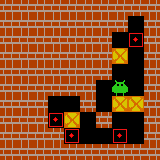
\includegraphics[width=0.35\textwidth]{assets/sokoban.png}
    \caption{Screenshot of the puzzle video game Sokoban. \cite{sokoban}}
    \label{fig:sokoban}
\end{figure}